\chapter*{Introduction}

The project is based on the paper 'Adaptation mechanisms 
in phosphorylation cycles by allosteric binding and gene 
autoregulation'. The aim of this paper was to study adaptation 
mechanics in a class of phosphorylation cycles under regulation 
by allosteric binding and gene autoregulation methods.

\section*{Mass Action Kinetics}
The paper has done all the math using the mass action kinetics 
which is described below.

\begin{definition}
    fFor the reaction $$\ce{E + S ->[k_f] P}$$
    The rate of reaction ($v$) is given by : 
    \begin{align*}
        v &= \frac{d[P]}{dt}\\
        &= k_f [E][S] 
    \end{align*}
\\
    This is known as the mass action kinetics.
\end{definition}

\section*{Michaelis-Menten Kinetics}

\noindent The project attempts to replicate the paper using 
Michaelis–Menten kinetics, which is defined as below.
\newpage
\begin{definition}
    fFor the reaction $$\ce{E + S <=>[k_f][k_b] ES ->[k_{cat}] P}$$
    The rate of reaction ($v$) is given by : 
    \begin{align*}
        v &= \frac{d[P]}{dt}\\
        &= V_{max} \frac{[S]}{[S] + K_d}
    \end{align*}
    \\

    In this, the definitions are as follows :
    \begin{align*}
        V_{max} &= k_{cat}[E]_0\\
        K_d &= \frac{k_b}{k_f}
    \end{align*}

    This is known as the Michaelis–Menten kinetics.
\end{definition}

\section*{Limitations of Michaelis–Menten Kinetics}

\noindent This is a different result as compared to mass 
action kinetics. The Michaelis–Menten kinetics operate under 
the assumption that $K_d \ll 1$, and in general operate under 
the rule that the second reaction is non reversible, which 
is applicable under the condition that $[S] \gg [P]$ or 
$\Delta G \ll 0$.
\\\\
Thus, the conditions under which Michaelis–Menten kinetics 
operate are :
\begin{itemize}
    \item $K_d \ll 1$
    \item $[S] \gg [P]$
    \item $\Delta G \ll 0$
\end{itemize}

\section*{Results of the Original Paper}
The original paper does mathematical analysis of the 
phosphorylation system given below :

\begin{center}
    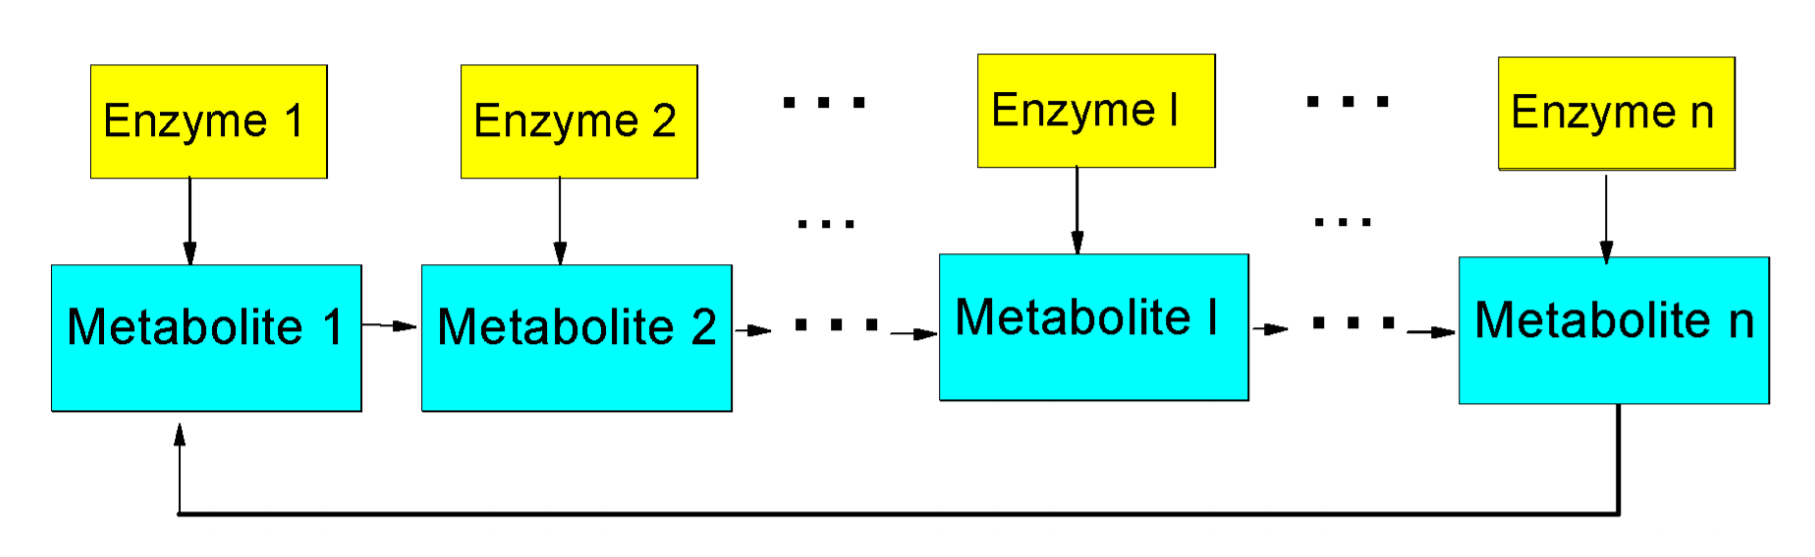
\includegraphics[scale=0.3]{img/orig-sys.png}
\end{center}

\noindent This system is described by the following 
set of equations :

$$ \ce{X_i + E_i <=>[K_{i,1}][K_i,2] X_iE_i -> X_{i+1} + E_i}$$

\noindent The paper then uses multiple Lemmas and 
Propositions to describe the behavior of the system. The 
following analyses are done on the system :

\begin{itemize}
    \item Robustness Analysis
    \item Stability Analysis
    \item Adaptation to Biological Rhythms
\end{itemize}

\noindent The aim of the project is to replicate results of 
the above analysis using Michaelis–Menten kinetics.